\documentclass[border=6pt]{standalone}
% ---------------------------------------------------------------------------
% tikzpreamble.tex -- shared by main.tex and by every standalone in tikz/
% ---------------------------------------------------------------------------
\usepackage{amsmath}
\usepackage{amssymb}
\usepackage{tikz}
\usepackage{circuitikz}
\usetikzlibrary{arrows.meta,calc,positioning,decorations.pathmorphing,decorations.pathreplacing,
                decorations.markings,patterns,angles,quotes,fit,
                shapes.geometric,shapes.misc,backgrounds,intersections}

\ctikzset{bipoles/length=0.85cm}
\ctikzset{resistors/scale=0.85}
\ctikzset{capacitors/scale=0.9}

\tikzset{
  wire/.style      = {line width=0.7pt},
  dashedwire/.style= {line width=0.7pt, densely dashed},
  term/.style      = {circle, draw, line width=0.6pt, fill=white,
                      inner sep=0pt, minimum size=4.5pt},
  node dot/.style  = {circle, fill=black, inner sep=0pt, minimum size=4pt},
  boxlabel/.style  = {font=\sffamily\small},
  annot/.style     = {font=\small, align=left},
  phasor/.style    = {-{Stealth[length=3.2mm,width=2.2mm]}, line width=1.1pt},
  thinphasor/.style= {-{Stealth[length=2.6mm,width=1.8mm]}, line width=0.7pt},
  axis line/.style = {-{Stealth[length=2.6mm,width=1.8mm]}, line width=0.6pt},
  guide/.style     = {densely dashed, line width=0.4pt, gray},
}
\usepackage{siunitx}

\begin{document}
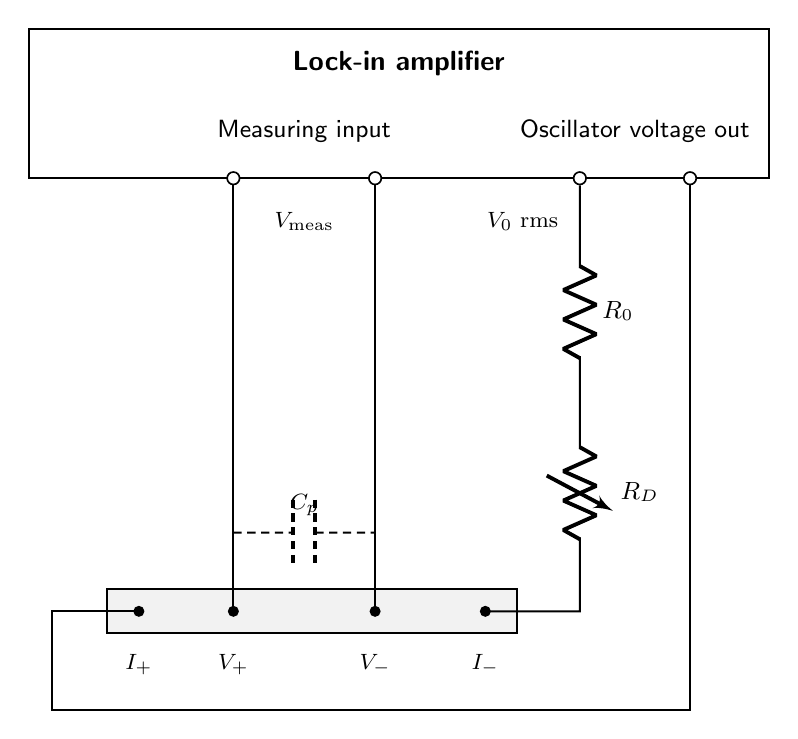
\begin{tikzpicture}[every node/.style={font=\small}]

  % ---- lock-in box -------------------------------------------------------
  \draw[wire] (0,0) rectangle (9.4,1.9);
  \node[boxlabel,font=\sffamily\bfseries] at (4.7,1.45) {Lock-in amplifier};
  \node[boxlabel] at (3.5,0.6) {Measuring input};
  \node[boxlabel] at (7.7,0.6) {Oscillator voltage out};

  % terminals
  \foreach \x in {2.6,4.4,7.0,8.4} { \node[term] at (\x,0) {}; }

  \node[font=\footnotesize] at (3.5,-0.55) {$V_{\mathrm{meas}}$};
  \node[font=\footnotesize,anchor=east] at (6.85,-0.55) {$V_0$ rms};

  % ---- sample ------------------------------------------------------------
  \draw[wire,fill=black!5] (1.0,-5.78) rectangle (6.2,-5.22);
  \foreach \x in {1.4,2.6,4.4,5.8} { \node[node dot] at (\x,-5.5) {}; }
  \node[font=\footnotesize,anchor=north] at (1.4,-5.92) {$I_{+}$};
  \node[font=\footnotesize,anchor=north] at (2.6,-5.92) {$V_{+}$};
  \node[font=\footnotesize,anchor=north] at (4.4,-5.92) {$V_{-}$};
  \node[font=\footnotesize,anchor=north] at (5.8,-5.92) {$I_{-}$};

  % ---- measuring leads ---------------------------------------------------
  \draw[wire] (2.6,-0.09) -- (2.6,-5.5);
  \draw[wire] (4.4,-0.09) -- (4.4,-5.5);

  % ---- parasitic capacitance (in parallel with the inner leads) ----------
  \draw[dashedwire] (2.6,-4.5) to[C] (4.4,-4.5);
  \node[font=\footnotesize] at (3.5,-4.15) {$C_p$};

  % ---- oscillator branch: R0 and RD in series ---------------------------
  \draw[wire] (7.0,-0.09) -- (7.0,-1.0)
              to[R=$R_0$] (7.0,-2.4)
              -- (7.0,-3.2)
              to[vR=$R_D$] (7.0,-4.8)
              -- (7.0,-5.5) -- (5.8,-5.5);

  % ---- return branch -----------------------------------------------------
  \draw[wire] (8.4,-0.09) -- (8.4,-6.75) -- (0.3,-6.75) -- (0.3,-5.5) -- (1.4,-5.5);
\end{tikzpicture}
\end{document}
